% !TEX TS-program = pdflatex
% !TEX encoding = UTF-8 Unicode

% This is a simple template for a LaTeX document using the "article" class.
% See "book", "report", "letter" for other types of document.

\documentclass[11pt]{report} % use larger type; default would be 10pt

\usepackage[utf8]{inputenc} % set input encoding (not needed with XeLaTeX)

%%% Examples of Article customizations
% These packages are optional, depending whether you want the features they provide.
% See the LaTeX Companion or other references for full information.

%%% PAGE DIMENSIONS
\usepackage{geometry} % to change the page dimensions
\geometry{a4paper} % or letterpaper (US) or a5paper or....
% \geometry{margin=2in} % for example, change the margins to 2 inches all round
% \geometry{landscape} % set up the page for landscape
%   read geometry.pdf for detailed page layout information

\usepackage{graphicx} % support the \includegraphics command and options

% \usepackage[parfill]{parskip} % Activate to begin paragraphs with an empty line rather than an indent

%%% PACKAGES
\usepackage{booktabs} % for much better looking tables
\usepackage{array} % for better arrays (eg matrices) in maths
\usepackage{paralist} % very flexible & customisable lists (eg. enumerate/itemize, etc.)
\usepackage{verbatim} % adds environment for commenting out blocks of text & for better verbatim
\usepackage{subfig} % make it possible to include more than one captioned figure/table in a single float
\usepackage{graphicx}
\usepackage{xcolor}
\usepackage{listings}
\lstset{basicstyle=\ttfamily,
  showstringspaces=false,
  commentstyle=\color{red},
  keywordstyle=\color{blue}
}

% These packages are all incorporated in the memoir class to one degree or another...

%%% HEADERS & FOOTERS
\usepackage{fancyhdr} % This should be set AFTER setting up the page geometry
\pagestyle{fancy} % options: empty , plain , fancy
\renewcommand{\headrulewidth}{0pt} % customise the layout...
\lhead{}\chead{}\rhead{}
\lfoot{}\cfoot{\thepage}\rfoot{}

%%% SECTION TITLE APPEARANCE
\usepackage{sectsty}
\usepackage{indentfirst}
\allsectionsfont{\sffamily\mdseries\upshape} % (See the fntguide.pdf for font help)
% (This matches ConTeXt defaults)

%%% ToC (table of contents) APPEARANCE
\usepackage[nottoc,notlof,notlot]{tocbibind} % Put the bibliography in the ToC
\usepackage[titles,subfigure]{tocloft} % Alter the style of the Table of Contents
\renewcommand{\cftsecfont}{\rmfamily\mdseries\upshape}
\renewcommand{\cftsecpagefont}{\rmfamily\mdseries\upshape} % No bold!

\makeatletter
\@addtoreset{section}{chapter}
\@addtoreset{subsection}{chapter}
\@addtoreset{subsubsection}{chapter}
\makeatother

%%% Font

%%% Spacing between paragraphs
\edef\restoreparindent{\parindent=\the\parindent\relax}
\usepackage{parskip}
\restoreparindent

%%% The "real" document content comes below...

\title{Supporting a Hadoop Cluster with IT Stock}
\author{Floriane Le Floch - Arthur Busser - Paul Dennetiere}
%\date{} % Activate to display a given date or no date (if empty),
         % otherwise the current date is printed 

\begin{document}

\maketitle
\renewcommand{\contentsname}{Summary}
\newpage
\tableofcontents
\newpage

\part{Introduction}
\part{Our solution}
\vspace*{\stretch{1}}
We want to make unused computers available for an Hadoop Cluster. In order to do that, we want to check at regular intervals if a computer is used or not (i.e. is in sleep mode). Our goal is to dynamically adding sleeping computer to the cluster, in order to make more ressources available.
In order to achieve this, we will have to ensure several things. This part will deals with the general structure, and what this structure induces for the cluster and added computers.
\vspace*{\stretch{1}}
\chapter{Setting up DataNodes on an unused computers}
First we will have to make the computer we want to add able to communicate with the Master (NameNode). We have several options to achieve this : \begin{itemize}
\item Virtualization
\item Use only linux distribution
\item Application containers
\end{itemize}
Only using linux distributions will greatly impact the interest of this project, so it's clearly not a solution. Virtualization doesn't seem good either, because of its need of ressources, and the general weight of those solutions. That's why we will use an Application Container : Docker.
\section{Docker}
Docker define itself as : \begin{quote}"Docker containers wrap up a piece of software in a complete filesystem that contains everything it needs to run: code, runtime, system tools, system libraries – anything you can install on a server. This guarantees that it will always run the same, regardless of the environment it is running in."\end{quote}

Therefore by using Docker we will be able to use a linux application on every operating system encountered in the company.
Moreover, by doing a snapshot of a running configuration, Docker allows us to deploy a solution very easily, and with a good velocity.
Finally, the global strategy is to have a "Slave Image" for Docker : 
Every computer of the company will have Docker installed on it, and will start Docker application every time the computer goes in sleep mode (we can easily do this through a C\# script, running in background, checking the sleep mode, and launching Docker application, or even using TaskLauncher included in Microsoft's OS).
\begin{figure}[ht!]
\centering
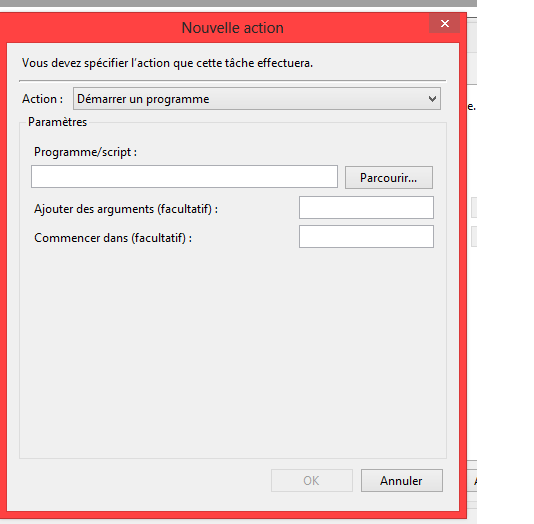
\includegraphics[width=90mm]{screen.png}
\caption{Screen of Microsoft's Task Launcher \label{overflow}}
\end{figure}
\section{Configuration}
We supposed that a "classical Hadoop cluster" is already configured (meaning we do not install a full cluster). So our goal is to provide Hadoop slave service on the computer, and to make it communicate with the Master.
We will first create an image of a running configuration. Such images are already available on Docker's Hub (Docker's image sharing website), but we will assume that we can't get such images : 
The first thing to do is to create a linux distributions image, a Debian for example. After that we install Hadoop slave service on this Debian.
\begin{itemize}
\item Creating Hadoop user and password : 

\begin{lstlisting}[language=bash]
useradd hadoop
passwd hadoop
\end{lstlisting}

\item Install Slave service on all slave by running on Master :
\begin{lstlisting}[language=bash]
# su hadoop 
$ cd /opt/hadoop 
$ scp -r hadoop hadoop-slave-1:/opt/hadoop 
$ scp -r hadoop hadoop-slave-2:/opt/hadoop
\end{lstlisting}
\item Setup Password less connectivity from master to new slave.
\begin{lstlisting}[language=bash]
mkdir -p $HOME/.ssh 
chmod 700 $HOME/.ssh 
ssh-keygen -t rsa -P '' -f $HOME/.ssh/id_rsa 
cat $HOME/.ssh/id_rsa.pub >> $HOME/.ssh/authorized_keys 
chmod 644 $HOME/.ssh/authorized_keys
scp $HOME/.ssh/id_rsa.pub hadoop@IPPATH:/home/hadoop/
\end{lstlisting}
Where IPPATH is the IP address of the new node.
And make the same thing on the slaves, in order to exchange ssh keys between master and slaves.

\item Then set a Hostname on new slaves in  /etc/sysconfig/network :
\begin{lstlisting}[language=bash]
NETWORKING=yes 
HOSTNAME=slaveX.in
\end{lstlisting}
Where X is the node Id (arbitrary setted, but unique)

\item Run on every new slave the following, to make changes effective : 
\begin{lstlisting}[language=bash]
hostname slaveX.in
\end{lstlisting}

\item Update /etc/hosts on all machines of the cluster with the following lines:
\begin{lstlisting}[language=bash]
IPPATH slaveX.in slaveX
\end{lstlisting}
\end{itemize}
By using this configuration we are able to dynamically add a data node to an existing cluster. The only point of failure is on IP addresses : every node should have a different one, and use it in order to have a functionnal network, however, this IP address can be found on the host.

Finally, the new slave have to start HDFS by using this command :
\begin{lstlisting}[language=bash]
./bin/hadoop-daemon.sh start datanode
\end{lstlisting}
This last command will have to be execute every time the docker application get started.

\section{Conclusion}
In conclusion, docker is a tool (application container) that will allow us to run hadoop on pretty much every system, and moreover allow us to have a configuration routine that pratically does not differ from a machine to another. By porting this solution on every computer of the company, we can assume that every computers going in sleep mode, and having a docker image configured like above, will connect to the master, and be part of the Hadoop cluster.

However we can easily imagine that many difficulties will come up, and we will discuss them in the following chapter.

\part{Difficulties that we expect to encounter}
\chapter{Redundancy Problems}
\section{What we expect to happen}
Because of bla bla blabla bla blabla bla blabla bla blabla bla blabla bla blabla bla blabla bla blabla bla blabla bla blabla bla bla

\end{document}
